\documentclass{article} % Denna måste vara med högst upp
\usepackage{graphicx} % Required for inserting images
\usepackage{amsmath}
\graphicspath{ {./Images/} }
\title{Kandidatarbete Ossian Jonathan}
\author{os7673er-s }
\date{21 April 2024}

\begin{document} % Denna måste också vara med för där man börjar dokumentet.

\maketitle{Inshallah}

\section{SectionTitle}
Kan man nu typ skriva text??? Wow ja det kan man!

Dota 2 is a 2013 multiplayer online battle arena (MOBA) video game by Valve. The game is a sequel to Defense of the Ancients (DotA), a community-created mod for Blizzard Entertainment's Warcraft III: Reign of Chaos. Dota 2 is played in matches between two teams of five players, with each team occupying and defending their own separate base on the map. Each of the ten players independently controls a powerful character known as a "hero" that all have unique abilities and differing styles of play. During a match players collect experience points and items for their heroes to defeat the opposing team's heroes in player versus player combat. A team wins by being the first to destroy the other team's "Ancient", a large structure located within their base.
$\frac{x^n-1}{x-1}$ % WTF den saken på den där intron ljög för oss, Man behöver tydligen ha det inbäddat i dollartecken.
$x_{2k}$







\subsection{Bishmillah}
Jonathan should play dota 2 with Ossian and Kevin and all the other boys ngl.

\begin{equation}
\frac{x^n-1}{x-1} = \sum_{k=0}^{n-1} x^k
\label{eqSum}
\end{equation}

\section{AYAYA} \label{poop}
We are who we are:





Detta hittar vi i ekvation \eqref{eqSum} som vi då ser där uppe


\begin{itemize}
\item AYAYA
\item gachiBASS
\end{itemize}



\label{name}
\ref{name} % JAG HAR INGEN ANING HUR DETTA FUNGERAR!?!?!



\begin{figure}
    \centering
    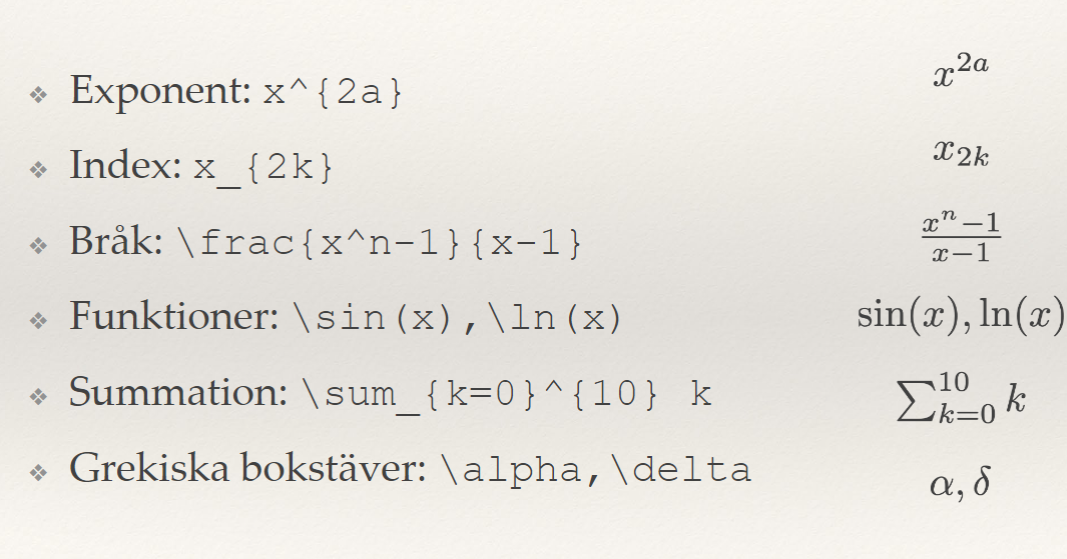
\includegraphics[width=0.6\linewidth]{randomImg.png}
    \caption{Enter Caption}
    \label{fig:enter-label}
\end{figure}

\section{yee i like it}
Vi kan se i sektion \ref{poop} att det går bra

\begin{figure}[h]
\begin{center}
\includegraphics[width=9cm]{Images/2MHZ_COMPARISON.png} %figurer sparas lämpligen i eps format
\caption{Exempel på figur. Det är viktigt att inte bara axlarna graderas utan att även storhet/enhet anges --- i detta fallet ''amplitud ($\mu$V)'' och ''tid (s)''. Undvik att använda automatskalning i Matlab!}
\label{figExempelSignal}
\end{center}
\end{figure}

\begin{figure}
     \centering
     \begin{subfigure}[b]{0.3\textwidth}
         \centering
         \includegraphics[width=\textwidth]{graph1}
         \caption{$y=x$}
         \label{fig:y equals x}
     \end{subfigure}
     \hfill
     \begin{subfigure}[b]{0.3\textwidth}
         \centering
         \includegraphics[width=\textwidth]{graph2}
         \caption{$y=3\sin x$}
         \label{fig:three sin x}
     \end{subfigure}
     \hfill
     \begin{subfigure}[b]{0.3\textwidth}
         \centering
         \includegraphics[width=\textwidth]{graph3}
         \caption{$y=5/x$}
         \label{fig:five over x}
     \end{subfigure}
        \caption{Three simple graphs}
        \label{fig:three graphs}
\end{figure}


\end{document}
